\section{Sustainability analysis}
The motivation behind this thesis is rooted in sustainability. Enabling the usage of coding techniques that can reduce power consumption on existing hardware aligns well with sustainability goal number 9 of the UN sustainable development goals: 'Build resilient infrastructure, promote inclusive and sustainable industrialization and foster innovation'. 

The UN sustainability goals are a set of goals that the entirety of the UN have adopted. It is a common framework used by the member nations to make better choices with respect to the environment, both physical and social. The goals include gender and racial equality as well as reducing emissions from industry.

Just like approximate computing is a tradeoff between precision and processing speed/power consumption, implementing \emph{all} of the sustainability goals requires making some tradeoffs between the difference categories. 

All the categories represent unquestionable quality of life improvements for all humans, though enacting them may result in contraticting results. For instance, goal 1 is to end poverty in all its forms everywhere. So a factory gets established, which creates several jobs for the empoverished residents at this location. However, the factory produces runoff that contaminates a nearby water source, going against goal number 6 of ensuring availability and sustainability of water and sanitation for all. 

The following analysis has been created using a lightweight version of SusAF (Sustainability Assessment Framework)~\cite{SusAF_website}. SusAF divides sustainability effects into 5 categories: Social, individual, technical, economic and environmental. The social aspect describes how the artifact under review affects interpersonal relationships, and the individual aspect describe changes in personal health and quality of life. The technical aspect concerns itself with the lifecycle of a product or service, and how the service can be adapted to changing needs or technical demands. The economic aspect describes how the artifact under review changes the business side of things, whether performing research or creating monetary value becomes easier or harder. Finally, the Environmental aspect describe how the artifact under review may affect nature, through increasing or decreasing the load on nature through human presence.

The artifact under review for this thesis is an analysis of reliability in approximate computing tools. The intended audience consists of approximate computing system developers and system architects looking to improve efficiency of their solution, and the analysis will be performed from their point of view. 

\subsection{Individual Impacts}
The biggest contribution on the individual plane is that the analysis may change a users perception of the reliability of approximate computing, and this could lead to implementing approximate computing in a hitherto untested area. 


\subsection{Social Impacts}
The same as for Individual Impacts...
\subsection{Environmental Impacts}
An analysis may facilitate the implementation of approximate computing in fields that can benefit from it. This results in lower resource usage if the output is not increased (e.g. performing larger simulations due to simulations being cheaper, thereby negating the positive effect of the system.

\subsection{Economic Impacts}
For product owners, approximate computing implementation may decrease costs of operation to produce an equivalent result. This in turn may trickle down to users of said program if price decreases due to the decrease in operation costs. 
Equally likely, the temptation of saving money may encourage service providers to accept risks now that they are more concrete in order to increase the cash flow.
\subsection{Technical Impacts}
Depending on what solution is implemented, the degree of maintainability of the program may decrease. This is due to having to understand the preexisting codebase, as well as understanding the transformations performed by the approximate computing program. 

If the approximate computing system is a drop-in tool, such as a compiler optimisation pass, in case of errors with the approximate computing tool it should be trivial to simply remove the optimisation pass, and the code should compile as usual.

This analysis does not delve into the scalability of approximate computing. This is further work.



Figure~\ref{fig:SusAF_diagram} shows how the different aspects of sustainability relate to each other. The numbers correspond to the entries in table~\ref{table:SusAF_table}. The arrows show in what direction the different sustainability outcomes may affect the other outcomes.

\todo[inline]{create table}

\begin{figure}
    \centering
    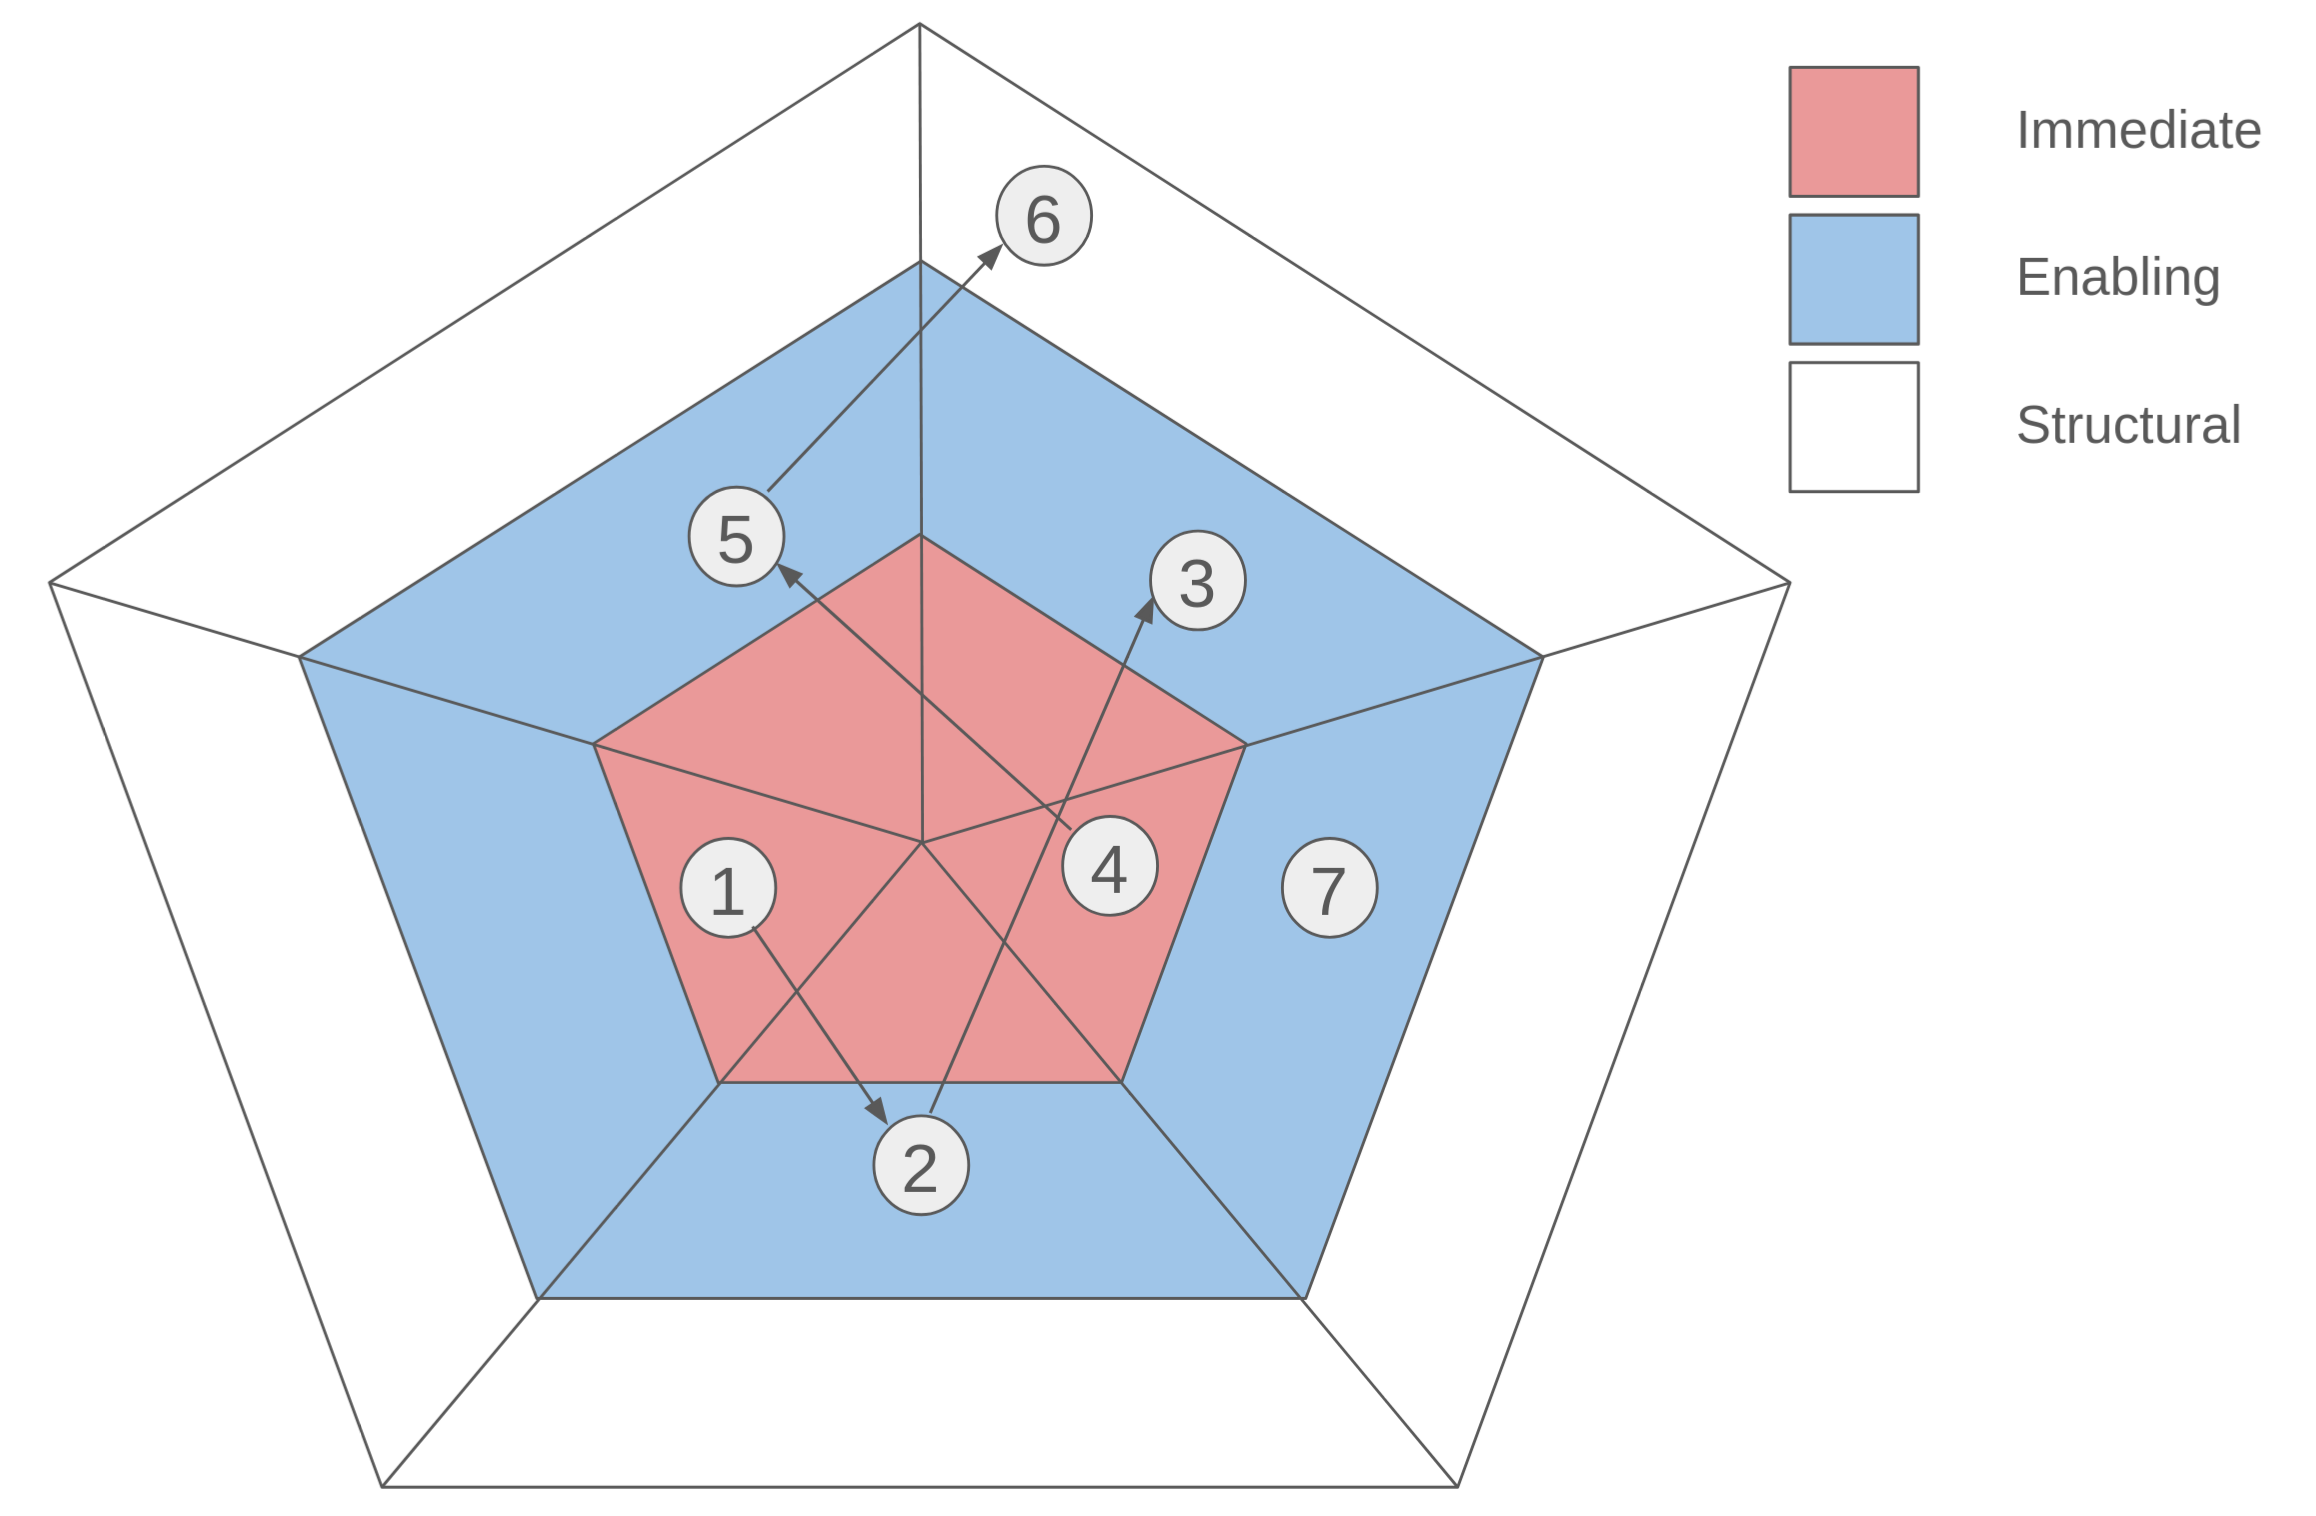
\includegraphics[width=0.5\linewidth]{Images/SusAF_diagram.png}
    \caption{A diagram of how different aspects of sustainability relate to each other}
    \label{fig:SusAF_diagram}
\end{figure}